\chapter*{6/6: Surfaces and Homology}
\addcontentsline{toc}{chapter}{6/6: Surfaces and Homology}

\section{Surfaces}

\begin{definition}[$n$-Manifold]
	 An \textit{$n$-manifold} is a topological space that locally looks like an open $n$-ball.
\end{definition}

\begin{example}
	\begin{enumerate}
		\item $S^1 = \{(x,y) \in \R^2 \mid x^2 + y^2 = 1\}$
        \begin{figure}[H]
            \centering
            \incfig[.2]{s1}
            \caption{$S^1$}
            \label{fig:s1}
        \end{figure}
        \item $S^2 = \{(x,y,z) \in \R^3 \mid x^2 + y^2 + z^2 = 1\}$
        \begin{figure}[H]
            \centering
            \incfig[.2]{s2}
            \caption{$S^2$}
            \label{fig:s2}
        \end{figure}
        \item $S^n = \{(x_1,x_2,\dots,x_n) \in \R^{n + 1} \mid x_1^2 + \dots + x_n^2 = 1\}$
        \item $T^2 = S^1 \times S^1$
        \begin{figure}[H]
            \centering
            \incfig[.2]{t2}
            \caption{$T^2$}
            \label{fig:t2}
        \end{figure}
        \item M\"obius Band (Mb).
        \begin{figure}[H]
            \centering
            \incfig[.2]{mobius-band}
            \caption{M\"obius Band}
            \label{fig:mobius-band}
        \end{figure}
        The M\"obius band is an example of a \textit{non-orientable} manifold. Also note, $\partial(\Mb) = S^1$. 
	\end{enumerate}
\end{example}

\begin{definition}[Connected Sum]
    To form the \textit{connected sum} of two surfaces, remove a disk from both surfaces and glue along the boundary of these disks:
    \begin{figure}[H]
        \centering
        \incfig[.5]{connected-sum}
        \caption{Connected Sum}
        \label{fig:connected-sum}
    \end{figure}
\end{definition}

\begin{definition}[Orientation]
    A surface is \textit{non-orientable} if there exists a circle on the surface such that a neighborhood of that circle on the surface is a M\"obius band.
\end{definition}

\begin{theorem}[Classification of Surfaces]
    Every orientable closed surface is homeomorphic to a genus g surface for some $g \geq 0$. Every non-orientable closed surface is homeomorphic to \[(\#^m\, \R P^2) \,\#\, (\#^n\, T^2),\] for $m > 0$ and $n \geq 0$.
\end{theorem}

\begin{example}
    The Klein bottle is given by $\R P^2 \# \R P^2$.
    \begin{figure}[H]
        \centering
        \incfig[.5]{the-klein-bottle}
        \caption{The Klein Bottle}
        \label{fig:the-klein-bottle}
    \end{figure}
\end{example}

\vspace{.5cm}
\section{Homology}

An $n$-manifold $M$ gives rise to $n$ abelian groups denoted $H_i(M)$ for $0 \leq i \leq n$. However, only those index by $0 < i < n$ are actually ``interesting''; as special cases, if $M$ has $m$ connected components, \[H_0(M) = \underbrace{\Z \oplus \dots \oplus \Z}_{\text{$m$ times}},\] and if $M$ is orientable, $H_n(M) = \Z$. In the case of surfaces, $H_i(M)$ are going to be finitely generated abelian groups, hence for some $s$ and $t$, \[H_i(M) = \Z^s \oplus \Z/p_1^{e_1}\Z \oplus \dots \oplus \Z/p_t^{e_t}\] where each $p_j$ is prime. Note also, $H_i(M)$ is invariant under homotopy equivalence.

\begin{example}
    \begin{enumerate}
        \item For $n = 1$, we have for $S^1$ that \[H_0(S^1) = \Z = H_1(S^1).\]
        \item For $n = 2$, we have for $\Sigma_g$ that \[H_0(\Sigma_g) = \Z = H_2(\Sigma_g),\] but what about $H_1(\Sigma_g)$. 
    \end{enumerate}
\end{example}

\vspace{.5cm}
\begin{definition}[Homology on Surfaces]$ $
    \begin{enumerate}
        \item Start by drawing a graph $G$ on a surface $\Sigma$ such that the edges are oriented in some way and $\Sigma \setminus G$ looks like the disjoint union of polygons (i.e. balls).
        \item Denote by $C_i$ the $i$-dimensional ``cells'' induced by this graph, so $C_0$ is the $\Z$-module $\Z\<v_1,\dots,v_V\>$ generated by the vertices of $G$, $C_1$ is $\Z\<e_1,\dots,e_E\>$ where the $e_i$ are edges of $G$, and $C_2$ is $\Z\<r_1,\dots,r_R\>$, where the $r_i$ are the $2$-dimensional regions bounded by the edges, i.e. the components of $\Sigma\setminus G$.
        \item Form the complex \[0 \to C_2 \xrightarrow{\partial_2} C_1 \xrightarrow{\partial_1} C_0 \to 0\] by defining the maps $\partial_1,\partial_2$ in the following way: send the generators of the codomain to linear combinations of the generators of the domain with coefficients determined by the orientations of the latter. For example, if we choose the standard counter-clockwise orientation on a region $r_i$, the coefficient of some $e_j$ is $1$ if the orientation ``agrees'' with that on $r_i$ and is $-1$ otherwise.
        \item Define $H_n(\Sigma) = \ker(\partial_n)/\im(\partial_{n + 1})$.
    \end{enumerate}
\end{definition}

\begin{example}
    Here we compute the homology of $S^1$.
	\begin{figure}[H]
		\centering
		\incfig[1]{cell-structure-on-s1}
		\caption{Cell structure on $S^1$}
		\label{fig:cell-structure-on-s1}
	\end{figure}
	So, we have that $C_0 = \Z\left< v_1,v_2 \right>$, $C_1 = \Z\left< e_1,e_2 \right>$, and $C_2 = \Z\left< r_1,r_2 \right>$ (in other words, three copies of $\Z \oplus \Z$). Looking at orientations, we find that \[0 \to \Z\left< r_1,r_2 \right> \xrightarrow{\partial_2} \Z\left< e_1,e_2 \right> \xrightarrow{\partial_1} \Z\left< v_1,v_2 \right> \to 0\] \[\partial_2 : \begin{cases}
			r_1 \mapsto e_2 - e_1\\
			r_2 \mapsto e_1 - e_2
		\end{cases}
		\quad
		\partial_1 : \begin{cases}
			e_1 \mapsto v_1 - v_2\\
			e_2 \mapsto v_1 - v_2
		\end{cases}
	\] So, $H_1(S^1) = 0$.
\end{example}

\vspace{.5cm}
\begin{problem}$ $
	\begin{enumerate}
		\item Compute $H_1(\Sigma_g)$ for all $g \geq 2$.
		\item Compute $H_1(\R P^2)$.
		\item Draw a closed loop $\gamma$ on the torus such that its homology class $[\gamma] = 4e_1 + 3e_2$.
	\end{enumerate}
\end{problem}
\begin{proof}$ $
	\begin{enumerate}
		\item Consider $\Sigma_g$ for $g \geq 2$. One way we can view $\Sigma_g$ is as the identification of edges of a $4g$-gon:
		\begin{figure}[H]
			\centering
			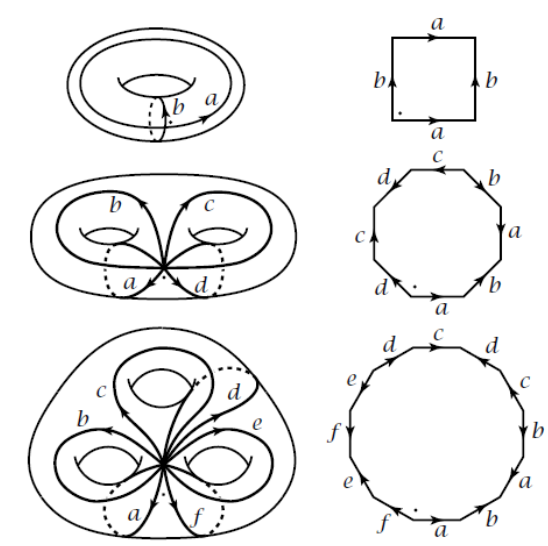
\includegraphics[scale=.3]{figures/genus-g-construction}
			\caption{Gluing edges of a $4g$-gon to construct a genus $g$ surface (Hatcher)}
			\label{fig:genus-g-construction}
		\end{figure}
		This is the cell structure we impose on $\Sigma_g$; namely, $C_0 = \Z\<v\>$ where $v$ is the single vertex under this identification, $C_1 = \Z\<e_1,\dots,e_{2g}\>$ where $e_1,\dots,e_{2g}$ are the edges connected to $v$ with their inherited orientation, and $C_2 = \Z\<r\>$ where $r \iso D^2$ is the interior of the polygon we started with. Then \[\partial_2(r) = e_1 - e_1 + e_2 - e_2 + \dots + e_{2g} - e_{2g} = 0\] and $\partial_1 = 0$, hence \[H_1(\Sigma_g) = \ker(\partial_1)/\im(\partial_2) = \Z^{2g}/0 = \Z^{2g}.\]
		\item We can compute $H_1(\RP^2)$ similarly. We can see $\RP^2$ as the identification of a square as follows:
		\begin{figure}[H]
			\centering
			\incfig[.2]{rp2-identification}
			\caption{$\RP^2$ Identification}
			\label{fig:rp2-identification}
		\end{figure}
		But of course, in this context, opposite edges on the square represent the same edge under the identification. Therefore, \[C_0 = \Z\left< v_1,v_2 \right>, \quad C_1 = \Z\left< e_1,e_2 \right>, \quad \text{and} \quad C_2 = \Z\left< r \right>\] and \[
			\partial_2: \begin{cases}
				r \mapsto 2e_1 + 2e_2
			\end{cases}
			\partial_1: \begin{cases}
				e_1 \mapsto v_1 - v_2\\
				e_2 \mapsto v_2 - v_1
			\end{cases}
		\] This gives us that \[H_1(\RP^2) = \ker(\partial_1)/\im(\partial_2) = \Z/2\Z.\]
		\item 
		\begin{figure}[H]
			\centering
			\incfig[.2]{closed-loop-homology}
			\caption{closed-loop-homology}
			\label{fig:closed-loop-homology}
		\end{figure}
	\end{enumerate}
\end{proof}

\section{Intersection Number}
\begin{figure}[H]
    \centering
    \incfig[.5]{intersection-straightened-out}
    \caption{Isotopy of a curve on a surface}
    \label{fig:intersection-straightened-out}
\end{figure}

\begin{definition}[Geometric Intersection Number]
	The \textit{geometric intersection number} between two curves $\gamma_1,\gamma_2$ on a surface $\Sigma$ is \[\iota(\gamma_1,\gamma_2) = \min\{\text{\# intersections of $\gamma_1,\gamma_2$}\}.\]
\end{definition}

\begin{definition}[Algebraic Intersection Number]
	The \textit{algebraic intersection number} is the pairing \[\gamma_1 \cdot \gamma_2 = \sum_{P \in \gamma_1 \cap \gamma_2} \mathcal{O}(P)\] where $\mathcal{O}(P)$ is the sign of the orientation on $P$ induced by the orientation of $\gamma_1,\gamma_2$.
\end{definition}

\begin{problem}
	How does $\gamma_1 \cdot \gamma_2$ change if
	\begin{enumerate}
		\item we reverse the orientation of $\gamma_1,\gamma_2$, or both?
		\item we reverse the orientation of $\Sigma$?
	\end{enumerate}
	Additionally, show that $\gamma_1 \cdot \gamma_2 = -\gamma_2 \cdot \gamma_1$.
\end{problem}
\begin{solution}
	\begin{enumerate}
		\item If we reverse the orientation of either $\gamma_1$ or $\gamma_2$, then $\gamma_1 \cdot \gamma_2$ changes by a sign. Thus, if we change both orientations, $\gamma_1 \cdot \gamma_2$ remains the same.
		\item Reversing the orientation of $\Sigma$ again changes $\gamma_1 \cdot \gamma_2$ by a sign.
	\end{enumerate}
\end{solution}


\begin{proposition}
	The algebraic intersection number gives a bilinear pairing $H_1(\Sigma) \times H_1(\Sigma) \to \Z$ defined by $\left< [\gamma_1], [\gamma_2] \right> \mapsto \gamma_1 \cdot \gamma_2$.
\end{proposition}

\begin{problem}
	Pick a basis for $H_1(\Sigma_2)$ and compute the intersection matrix.
\end{problem}
\begin{solution}
	Suppose that $H_1(\Sigma_2)$ has basis given by $\{[e_i]\}_{i = 1}^4$, where the $e_i$ are the same curves identified in the computation of $H_1(\Sigma_g)$. Then the intersection matrix is given by \[ \begin{pmatrix} e_i \cdot e_j \end{pmatrix} = \begin{pmatrix}  \end{pmatrix}  \] 
\end{solution}

